\documentclass{article}
\usepackage{graphicx}
\usepackage{hyperref}
\usepackage{float}
\usepackage{caption}
\usepackage{pdfpages}

\title
{
	Practica 5 \\
	Algoritmos de Busqueda Parte 2
}

\author
{
	Adolfo Roman Jimenez
}

\begin{document}
	
	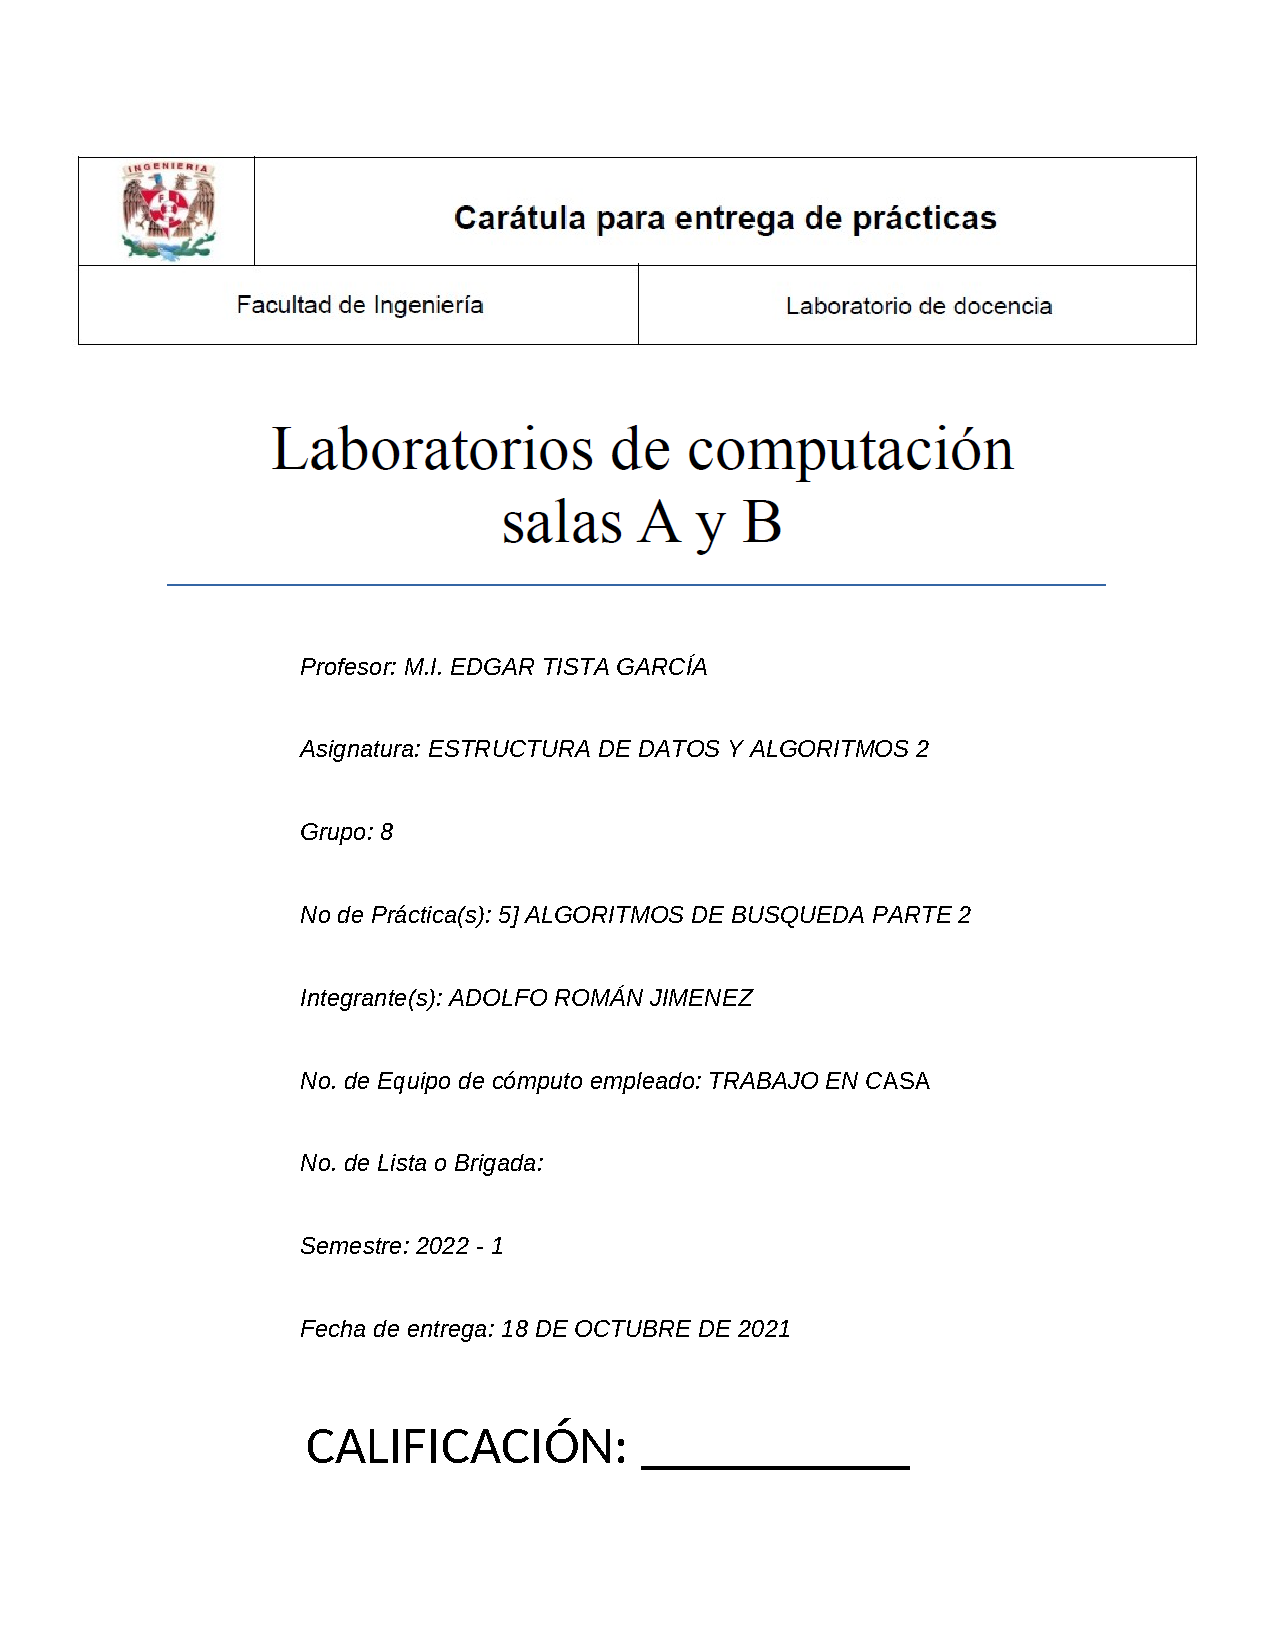
\includepdf[pages=-]{c5.pdf}
	
	\maketitle
	
	\section{Objetivo}
		
		El estudiante conocerá e identificará las características necesarias para realizar búsquedas por transformación de llaves.
		
	\section{Objetivo de Clase}
		
		El alumno conocerá la implementación de la transformación de llaves en el
		lenguaje orientado a objetos.
		
	\newpage
		
	\section{Ejercicio 0: Menu para la practica}
	
		\subsection{Desarrollo}
		
			Para el primer ejercicio el desarrollo fue muy sencillo. Como la practica lo indica, primeramente cree el proyecto en \textit{Java} con el nombre de \textbf{Practica5[RomanAdolfo]} y despues procedi a crear la clase prinicipal del proyecto que tambien lleva por nombre \emph{Practica5}.\\
			
			Esta clase es la unica que contiene a la funcion principal, mientras que todas las demas clases no contienen ninguna.\\
			
			A continuacion, como la practica lo indicaba, procedi a crear el menu del usuario con las opciones requeridas y una adicional para salir del programa.
			
			\begin{enumerate}
				\item Manejo de Tablas Hash en Java
				\item Función hash por módulo
				\item Encadenamiento
				\item Salir
			\end{enumerate}
		
			Al principio de la clase se declara \verb|import java.util.Scanner;| para poder hacer uso del \textit{Scanner} posteriormente. Ya dentro del la funcion principal se crea una nueva instancia \textbf{scan} del \textit{Scanner} y una variable entera \textbf{option}, que almacenara la opcion deseada para navegar en el menu.\\
			
			Por dentro el menu se compone de dos \textit{do-while} loops indexados, que rompen el ciclo, el primero cuando se escoje la opcion indicada dentro del menu y el segundo, cuando se escoje la opcion numero 4 que es la que permite al usuario terminar el programa.\\
			
			Despues de que el usuario escoje alguna opcion valida, entre a una estructura \textit{switch} que contiene 3 casos entre los que se encuentra el codigo de los ejercicios que se fueron creando durante la practica.
		
		\subsection{Ejecucion}
		
			\begin{figure}[H]
				\centering
				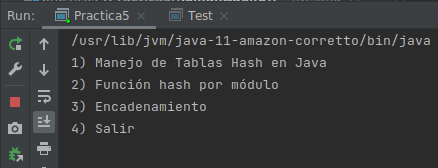
\includegraphics[scale=0.9]{images/e0.png}
				\caption*{Ejercicio 0: Menu Principal}
			\end{figure}
			
			\newpage
									
	\section{Ejercicio 1: Tablas Hash en Java}
	
		\subsection{Desarrollo}
		
			Cuando el usuario ingresa la opcion numero 1 en el menu principal, la estructura \textit{switch} lo llevara al codigo escrito para el ejercicio de las tablas hash.\\
			
			Para este ejercicio se creo una nueva clase llamada \emph{HashTable} que al principio del codigo, declara importa la clase \verb|import java.util.HashMap;|. Esta clase se usa para crear una tabla hash por medio de la clase \emph{HashMap} para la cual en un inicio, le asignamos un dato de tipo entero como \textit{key} y otro de tipo \textit{string} como \textit{value} y a la nueva instancia de la \emph{HashMap} le ponemos el nombre de \textbf{stdlist}.\\
			
			La clase \emph{HashTable} tambien contiene un menu interno que esta declarado en forma de metodo de la clase llamado \emph{hashMenu()}.\\
			
			Cuando el usuario en el menu principal escoje la opcion numero 1, la estructura \textit{switch} en el caso uno, primero crea una nueva instancia de la clase \emph{HashTable} a la cual le asigna el nombre de \textbf{stdHash} y acto seguido, penetra en la instancia a traves del metodo \emph{hashMenu()} que interactua con todos los metodos internos de la clase para llevar a cabo su proposito.\\
			
			El menu de el metodo \emph{hashMenu()} es el siguiente:
		
			\begin{figure}[H]
				\centering
				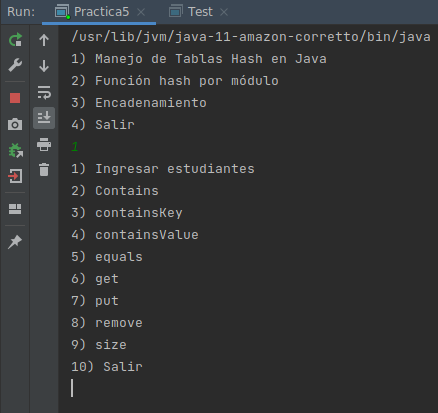
\includegraphics[scale=0.5]{images/e1.png}
				\caption*{Ejercicio 1: Menu Principal}
			\end{figure}
		
		Explicaremos cada uno de estos metodos y que es lo que hacen:\\
		
			\subsubsection{Ingresar Estudiantes}
			
				Cuando en este menu, el usuario escoje la opcion numero 1, el programa lo mandara al metodo privado \emph{insertStudents()}. Dentro de este metodo, primeramente y a traves de una leyenda se le solicita al usuario que ingrese la cantidad de estudiantes que desea agregar; para capturar esta informacion se declara la variable entera \textbf{number} y se escanea el numero que el usuario desee ingresar.\\
				
				Acto seguido, a traves de un \textit{while-loop} que iterara la cantidad de veces que el usuario en \textbf{number} haya declarado, se invocara al metodo \emph{insertStd()}.\\
				
				El metodo \emph{insertStd()}, tambien privado, en el momento en el que el usuario ingresa a el, se le pregunta por medio de una impresion en pantalla que inserte el nombre del alumno. A traves de una variable global de tipo \textit{String} llamada \textbf{name} y con ayuda del metodo \emph{useDelimiter()} en la instancia \emph{scan()} que permite incluir espacios dentro del \textit{input} del usuario, se deposita la informacion en \textbf{name}.\\
				
				Posteriormente, el programa tambien pide que se ingrese el numero de cuenta del usuario y este se deposita en la variable entera \textbf{key}.\\
				
				Cuando se ha terminado de ingresar los dos valores, a traves del metodo \emph{stdlist.put()} se ingresan los parametros \textbf{key} en primer lugar y \textbf{name} en segundo lugar que correponden a la llave y al valor en la tabla hash.\\
				
				En el ejercicio, esto lo llevamos a cabo diferentes veces con los siguientes nombres:
				
				\begin{figure}[H]
					\centering
					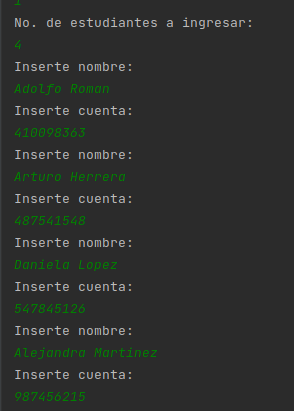
\includegraphics[scale=0.8]{images/e12.png}
					\caption*{Ejercicio 1: Captura de nombres}
				\end{figure}
			
			\subsubsection{Contains}
			
				Una vez que los nombres han sido capturados, pasamos a la opcion numero 2 que corresponde con el metodo \emph{containing()}.\\
				
				En este metodo, a traves de la funcion \emph{isEmpty()} se evalua que la table no este vacia, si no lo esta.		
	
		
		\subsection{Ejecucion}
			
			
			\begin{figure}[H]
				\centering
				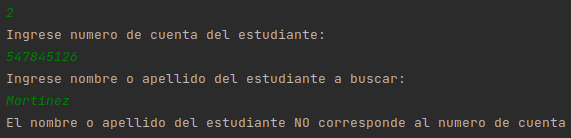
\includegraphics[scale=0.6]{images/e13.png}
				\caption*{Ejercicio 1: Opcion 2}
			\end{figure}
			
			\begin{figure}[H]
				\centering
				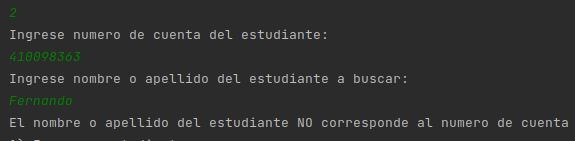
\includegraphics[scale=0.6]{images/e14.png}
				\caption*{Ejercicio 1: Opcion 2}
			\end{figure}
			
			\begin{figure}[H]
				\centering
				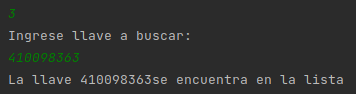
\includegraphics{images/e15.png}
				\caption*{Ejercicio 1: Opcion 3}
			\end{figure}
			
			\begin{figure}[H]
				\centering
				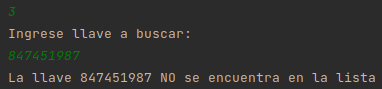
\includegraphics{images/e16.png}
				\caption*{Ejercicio 1: Opcion 3}
			\end{figure}
			
			\begin{figure}[H]
				\centering
				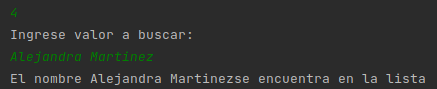
\includegraphics{images/e17.png}
				\caption*{Ejercicio 1: Opcion 4}
			\end{figure}
			
			\begin{figure}[H]
				\centering
				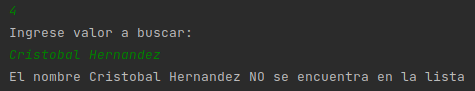
\includegraphics{images/e18.png}
				\caption*{Ejercicio 1: Opcion 4}
			\end{figure}
			
			\begin{figure}[H]
				\centering
				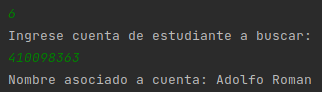
\includegraphics{images/e19.png}
				\caption*{Ejercicio 1: Opcion 6}
			\end{figure}
			
			\begin{figure}[H]
				\centering
				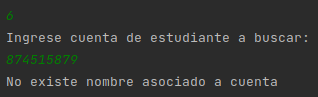
\includegraphics{images/e110.png}
				\caption*{Ejercicio 1: Opcion 6}
			\end{figure}
			
			\begin{figure}[H]
				\centering
				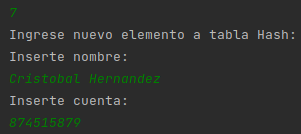
\includegraphics{images/e111.png}
				\caption*{Ejercicio 1: Opcion 7, ingresando nuevo elemento}
			\end{figure}
			
			\begin{figure}[H]
				\centering
				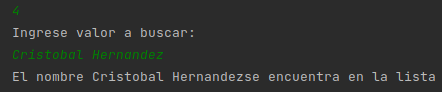
\includegraphics{images/e112.png}
				\caption*{Ejercicio 1: Opcion 4, buscando nuevo elemento}
			\end{figure}
			
			\begin{figure}[H]
				\centering
				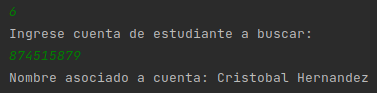
\includegraphics{images/e113.png}
				\caption*{Ejercicio 1: Opcion 6, buscando nuevo elemento}
			\end{figure}
			
			\begin{figure}[H]
				\centering
				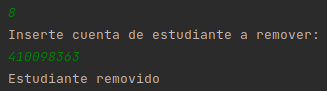
\includegraphics{images/e114.png}
				\caption*{Ejercicio 1: Opcion 8}
			\end{figure}
			
			\begin{figure}[H]
				\centering
				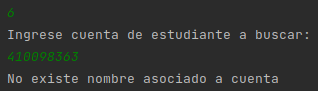
\includegraphics{images/e115.png}
				\caption*{Ejercicio 1: Opcion 6, buscando elemento removido}
			\end{figure}
			
			\begin{figure}[H]
				\centering
				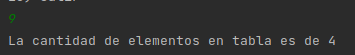
\includegraphics{images/e116.png}
				\caption*{Ejercicio 1: Opcion 9}
			\end{figure}
			
			\begin{figure}[H]
				\centering
				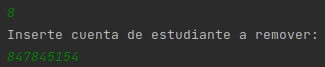
\includegraphics{images/e117.png}
			\caption*{Ejercicio 1: Opcion 8, removiendo elementos}
			\end{figure}
			
			\begin{figure}[H]
				\centering
				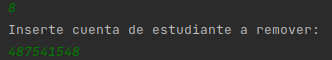
\includegraphics{images/e118.png}
				\caption*{Ejercicio 1: Opcion 8, removiendo elementos}
			\end{figure}
			
			\begin{figure}[H]
				\centering
				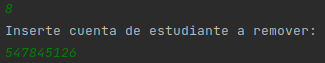
\includegraphics{images/e119.png}
				\caption*{Ejercicio 1: Opcion 8, removiendo elementos}
			\end{figure}
			
			\begin{figure}[H]
				\centering
				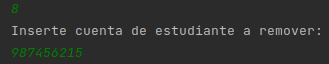
\includegraphics{images/e120.png}
				\caption*{Ejercicio 1: Opcion 8, removiendo elementos}
			\end{figure}
			
			\begin{figure}[H]
				\centering
				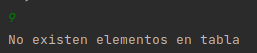
\includegraphics{images/e121.png}
				\caption*{Ejercicio 1: Opcion 9, no existen elementos}
			\end{figure}
		
			
			\begin{figure}[H]
				\centering
				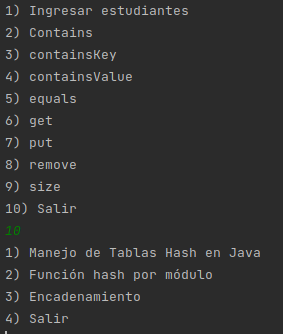
\includegraphics{images/e123.png}
				\caption*{Ejercicio 1: Opcion 10, salida del programa}
			\end{figure}
			
			\newpage

	\section{Ejercicio 2}
	
		\subsection{Desarrollo}
		
			Cuando el usuario en el menu principal escoge la opcion numero 2, entonces se dirigira al codigo escrito dentro de la clase \emph{HaskModulo}.\\
			
			La clase \emph{HashModulo} es una clase cuyo objetivo es demostrar la forma en la que se puede usar una funcion \textit{hash} para almacenar elementos en un arreglo regular a traves de una funcion sencilla que permita encontrar a estos elementos rapidamente cada vez que se les busque.\\
			
			Para lograr esto, primeramente la clase usa el codigo \verb|import java.util.LinkedList;| para poder hacer uso de las listas ligadas para el funcionamiento del programa.\\
			
			Cuando ingresamos a la clase, lo primero que haremos sera crear una lista ligada de variables enteras a la cual le llamaremos \textbf{lst}.\\
			
			El constructor de esta clase, que lleva el mismo nombre, carece de parametros iniciales, pero dentro del cuerpo de su metodo yace un \textit{for-loop} que itera 20 veces como el ejercicio lo requiere y agrega unicamente \textit{null} a cada uno de los indices del arreglo.\\
			
			El menu contiene los elementos requeridos por el ejercicio, que son las acciones de \textbf{Ingresar elementos}, \textbf{Imprimir lista} y \textbf{Buscar elementos} como se muestra en la siguiente imagen.\\
			
			\begin{figure}[H]
				\centering
				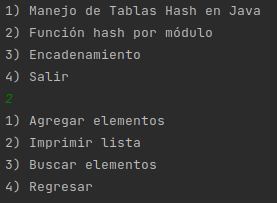
\includegraphics[scale=0.9]{images/e21.png}
				\caption*{Ejercicio 2: Menu Principal}
			\end{figure}
		
			Dependiendo de la opcion que el usuario elija, lo llevara a la opcion correspondiente.\\
			
			Para la opcion numero 1, lo dirigimos al metodo \emph{addElement()}.\\
			
			El metodo \emph{addElement()}, utiliza algunas funciones auxiliares. Primeramente solicita al usuario que ingrese el elemento deseado y este se deposita en la variable enterea \textbf{val}, despues de esto, como sabemos que \textbf{val} debe de tener un numero entero de 9 digitos que representa un numero de cuenta, entonces procedemos a obtener la suma de sus digitos a traves del metodo \emph{folding()}.\\
			
			Dentro del metodo \emph{folding()} que es un metodo que devuelve un entero, declaramos una variable entera \textbf{sum} y acarreamos como argumento el entero \textbf{val} que contiene al numero de cuenta.\\
			
			Para poder hacer uso de la tecnica de \textit{folding}, procedemos a lo siguiente. 
			
			\begin{itemize}
				\item Depositamos en \textbf{sum} el modulo 10 de var
				\item Dividimos sobre 10 a \textbf{var} y reasignamos su propio valor
				\item Con un \textit{for-loop} obtenemos el modulo de \textbf{var} sobre 10,000 y lo sumamos a \textbf{sum}
				\item Dividimos a \textbf{var} sobre 10,000 y reasignamos su propio valor
				\item Repetimos este proceso 2 veces
				\item Regresamos el valor en \textbf{sum}
			\end{itemize}
		
			A traves de este proceso, el numero de cuenta se divide en 2 conjuntos de 4 digitos y 1 de 1, los cuales se suman para obtener el valor en \textbf{sum} que despues se transfiere de igual forma.\\
			
			Al momento de recibir el resultado, el metodo \emph{addElement()} procede a invocar al metodo \emph{probing()} que incluye a los argumentos \textbf{var} que contiene el numero de cuenta y \textbf{sum} que contiene el resultado del \textit{folding} del numero de cuenta.\\
			
			Para \emph{probing()} el proceso es un poco mas sencillo ya que simplemente se hace uso de la formula para \textit{probing} que es la siguiente:
			
			
			\begin{figure}[H]
				\centering
				$h'(x)= (h(x) + f(i)) \% n$ 
				\newline
				\centering
				$h(x)= x \% n$
				\newline
				\centering
				$f(i)= 0,1,2,3...$ 
				\newline
			\end{figure}
		
			Cuando nosotros usamos el \textit{for-loop} para ingresar los elementos a la lista ligada, asignamos una variable de tipo entero \textbf{index} dentro de la cual, depositamos el modulo 20 de la variable \textbf{sum} mas el valor en \textbf{i} del iterador, de nuevo entre el modulo 20.\\
			
			Esto constantemente nos propociona indices que se encuentran dentro del arreglo y continua su ejecucion hasta que el metodo es capaz de colocar un elemento dentro del arreglo.\\
			
			Cuando existe colision, esto es, cuando el indice dentro del que se quiere ingresar el \textbf{val} no es igual a \textit{null}, entonces continua el \textit{for-loop} hasta un maximo de 20 veces, pues es la cantidad de espacios disponibles.\\
			
			El \textit{for-loop} se rompe, en el momento en que un valor logra colocarse dentro del arreglo y este imprime una leyenda inidicado el valor colocado y el indice. 
		
		\subsection{Ejecucion}

			\begin{figure}[H]
				\centering
				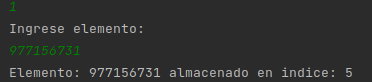
\includegraphics{images/e22.png}
				\caption*{Ejercicio 2: Colocando elementos dentro del arreglo}
			\end{figure}
			
			\begin{figure}[H]
				\centering
				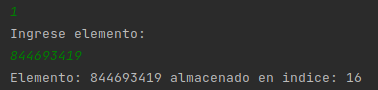
\includegraphics{images/e23.png}
				\caption*{Ejercicio 2: Colocando elementos dentro del arreglo}
			\end{figure}
			
			\begin{figure}[H]
				\centering
				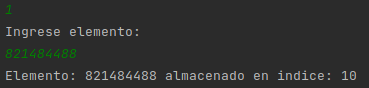
\includegraphics{images/e24.png}
				\caption*{Ejercicio 2: Colocando elementos dentro del arreglo}
			\end{figure}
			
			\begin{figure}[H]
				\centering
				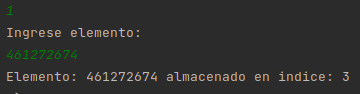
\includegraphics{images/e25.png}
				\caption*{Ejercicio 2: Colocando elementos dentro del arreglo}
			\end{figure}
			
			\begin{figure}[H]
				\centering
				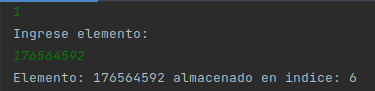
\includegraphics{images/e26.png}
				\caption*{Ejercicio 2: Colocando elementos dentro del arreglo}
			\end{figure}
			
			\begin{figure}[H]
				\centering
				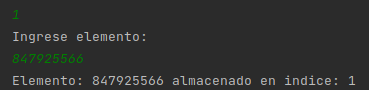
\includegraphics{images/e27.png}
			\caption*{Ejercicio 2: Colocando elementos dentro del arreglo}
			\end{figure}
			
			\begin{figure}[H]
				\centering
				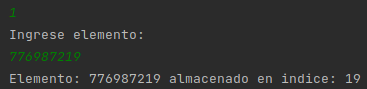
\includegraphics{images/e28.png}
				\caption*{Ejercicio 2: Colocando elementos dentro del arreglo}
			\end{figure}
			
			\begin{figure}[H]
				\centering
				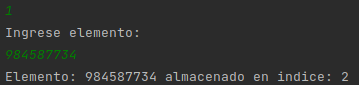
\includegraphics{images/e29.png}
			\caption*{Ejercicio 2: Colocando elementos dentro del arreglo}
			\end{figure}
			
			\begin{figure}[H]
				\centering
				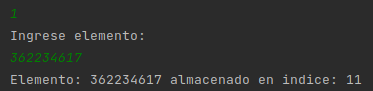
\includegraphics{images/e210.png}
				\caption*{Ejercicio 2: Colocando elementos dentro del arreglo}
			\end{figure}
			
			\begin{figure}[H]
				\centering
				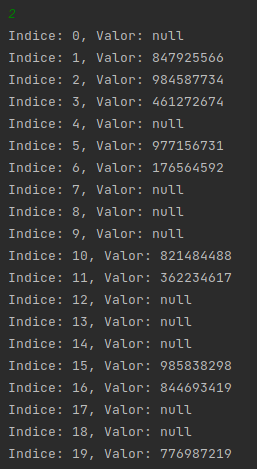
\includegraphics{images/e211.png}
				\caption*{Ejercicio 2: Impresion de elementos dentro de la lista}
			\end{figure}
			
			\begin{figure}[H]
				\centering
				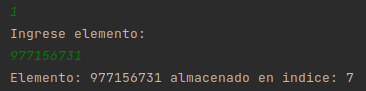
\includegraphics{images/e212.png}
				\caption*{Ejercicio 2: Colocando elemento repetido dentro del arreglo}
			\end{figure}
			
			\begin{figure}[H]
				\centering
				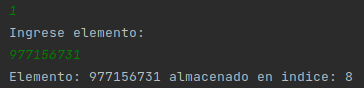
\includegraphics{images/e213.png}
				\caption*{Ejercicio 2: Ingresando elemento repetido}
			\end{figure}
			
			\begin{figure}[H]
				\centering
				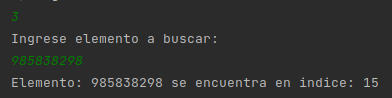
\includegraphics{images/e214.png}
				\caption*{Ejercicio 2: Buscando elementos dentro del arreglo}
			\end{figure}
			
			\begin{figure}[H]
				\centering
				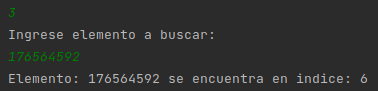
\includegraphics{images/e215.png}
				\caption*{Ejercicio 2: Buscando elementos dentro del arreglo}
			\end{figure}
			
			\begin{figure}[H]
				\centering
				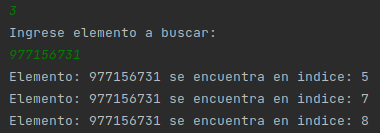
\includegraphics{images/e216.png}
				\caption*{Ejercicio 2: Buscando elemento repetido dentro de arreglo}
			\end{figure}
			
			\begin{figure}[H]
				\centering
				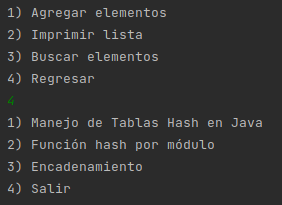
\includegraphics{images/e217.png}
				\caption*{Ejercicio 2: Salida del programa}
			\end{figure}
			
			\newpage

	\section{Ejercicio 3}
	
		\subsection{Desarrollo}
		
			Por ultimo, para cuando el usuario en el menu principal ingresa la opcion numero 3, a traves del \textit{switch} el usuario ingresara al caso 3 que corresponde al codigo de la clase \emph{Encadenamiento}.
			
			Como en las ocasiones anteriores, primero se crea una nueva instancia de la clase llamada \textbf{lstEncad} y despues se ingresa en uno de los metodos de esa instancia que tambien lleva al menu principal a traves del metodo \emph{menuEncadenamiento()}.\\
			
			La clase \emph{Encadenamiento} corresponde al ejercicio de "lista de listas" y es por esta razon que al principio de la clase se declaran distintas clases para importar como lo son:
			
			\begin{itemize}
				\item \verb|import java.util.ArrayList;|
				\item \verb|import java.util.List;|
				\item \verb|import java.util.Random;|
			\end{itemize}
		
			Las primera \emph{ArrayList} nos servira para la lista de enteros que queremos crear, mientra que la segunda \emph{List} nos funcionara para hacer la lista principal que contendra a las demas listas. 
			
			La clase \emph{Random} nos servira para poder realizar lo que el ejercicio pide, ya que con ella generaremos numeros al azar para poder ingresar elementos en posiciones al azar como el ejercicio lo marca.
			
			Una vez que hemos ingresado a la clase, lo primero que encontramos es la declaracion de una \emph{List} cuyos elementos son del tipo \emph{ArrayList<Integer>} que es una sublista que contiene variables enteras. A esta lista principal le llamamos \textbf{masterList}.
			
			Despues de crear las instancias requeridas tanto de \emph{Random} como de \emph{Scanner} para su uso posterior, pasamos al constructor de la clase \emph{Encadenamiento}.
			
			El constructor de la clase es uno que no tiene parametros, pero dentro de su cuerpo encontramos un \textit{for-loop} que itera 15 veces de acuerdo a lo requerido por el ejercicio y cada vez que lo hace, creara una lista de enteros \emph{ArrayList<>} a que tendra como nombre \textbf{sublista} y acto seguido a traves del metodo \emph{add()} en \textbf{masterList} agregara esa lista creada por cada iteracion.\\
			
			Cabe mencionar que a pesar de que la lista generada \textbf{sublista} siempre tiene el mismo nombre, por cada nueva instancia creada, el programa en realidad crea un objeto distinto dentro de la memoria con un numero de referencia distinto que apunta a otro objeto y no al mismo. Caso contrario, si hubieramos creado una instancia \textit{antes} de ingresar al \textit{for-loop} y esa misma instancia de lista la hubieramos ingresado 15 veces a \textbf{masterList} entonces simplemente habriamos ingresado 15 veces la misma referencia al mismo objeto, por lo cual cada elemento agregado en esa referencia, seria el mismo para "todas las demas" pues la referencia seria la misma.\\
			
			Esto solo es el constructor, para el menu, como el ejercicio lo solicita, unicamente agregamos 2 opciones que son:
			
			\begin{enumerate}
				\item Agregar elementos
				\item Salir
			\end{enumerate}
		
			Dependiendo de la opcion que el usuario elija, sera lo que el programa realice, pero si escoge la opcion 1, entonces el programa lo mandara hacia el metodo \emph{allTheStuffThisDoes()} que contiene un par de metodos adicioneales los cuales son \emph{addElement()} y \emph{print()}.\\
			
			El metodo \emph{addElement()} primeramente solicita al usuario textualmente el elemento a agregar.\\
			
			Por medio de una variable entera \textbf{element} se captura el elemento que el usuario desee agregar. Despues de esto, se declara la variable entera \textbf{index} la cual se auxilia de la instancia de la clase \emph{Random} para formular un numero al azar entre 0 y 14, lo que corresponde a la cantidad de indices disponibles dentro de la \textbf{masterList}.\\
			
			Acto seguido, se usan dos metodos en \textbf{masterList} para ingresar el elemento en el la lista correspondiente al indice requerido.\\
			
			Primero se usa el metodo \emph{get()} al cual se agrega como parametro la variable en \textbf{index} lo que nos devuelve la lista en el indice que se encuentre en \textbf{index}, despues de eso usamos el metodo \emph{add()} que usa de parameto el elemento en \textbf{element} para agregar ese elemento a la lista que corresponda al indice en \textbf{index}.\\
			
			Es asi como se ingresan los elementos al azar en las listas.\\
			
			Despues de esto hacemos uso de el metodo \emph{print()} el cual dentro de su cuerpo, simplemente itera a traves de cada uno de los indices de \textbf{masterList} los cuales corresponde a cada una de las listas de enteros que esta contiene y despues por medio del metodo \emph{System.out.println()} en forma estructurada, se indica cual es el numero de lista que se esta imprimiendo y los contenidos de esta. Esto sucede cada momento despues de que se agrega un elemento para ir mostrando como va progresando este codigo.\\
			
			Al finalizar el programa, simplemente regresa al menu principal de la clase \emph{Encadenamiento} y el usuario es quien decide si continua ingresando elementos o usa la opcion 2 para salir de la instancia de clase.
		
		\subsection{Ejecucion}
		
		En las siguientes imagenes, se muestra la ejecucion de la clase \emph{Encadenamiento}.\\

			\begin{figure}[H]
				\centering
				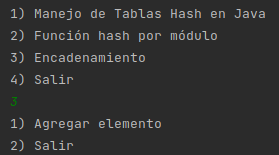
\includegraphics{images/e31.png}
				\caption*{Ejercicio 3: Menu Principal}
			\end{figure}
			
			\begin{figure}[H]
				\centering
				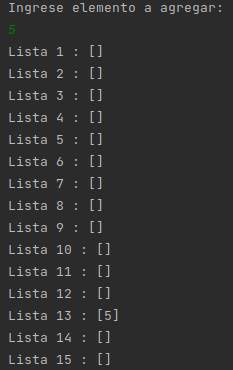
\includegraphics{images/e32.png}
				\caption*{Ejercicio 3: Opcion 1, se agrega elemento 5}
			\end{figure}
			
			\begin{figure}[H]
				\centering
				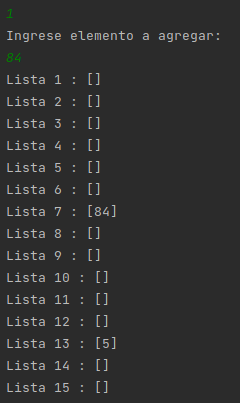
\includegraphics{images/e33.png}
				\caption*{Ejercicio 3: Opcion 1, se agrega elemento 84}
			\end{figure}
			
			\begin{figure}[H]
				\centering
				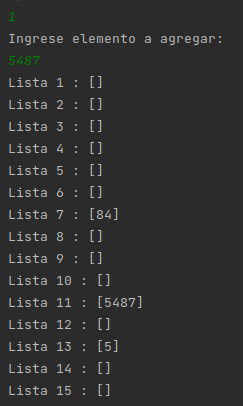
\includegraphics{images/e34.png}
				\caption*{Ejercicio 3: Opcion 1, se agrega elemento 5487}
			\end{figure}
			
			\begin{figure}[H]
				\centering
				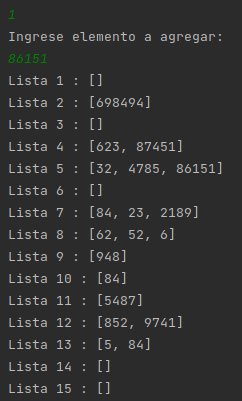
\includegraphics{images/e35.png}
				\caption*{Ejercicio 3: Despues de agregar diferentes elementos}
			\end{figure}
			
			\begin{figure}[H]
				\centering
				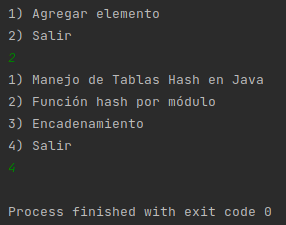
\includegraphics{images/e36.png}
				\caption*{Ejercicio 3: Opcion 2, finalizacion del programa}
			\end{figure}
			
			\newpage

	
	\section{Conclusiones}
	
	Esta practica estuvo interesante, porque me ayudo a entender como implementar una funcion \textit{Hash Table} en Java, algo que pienso ni si quiera intentado en C anteriormente.\\
	
	Me parece que en \textit{Python} ya la habia usado y creo que es este tipo de dato al que le llaman \textit{Dictionary}, el cual sinceramente siempre me parecio bastente practico, pero que cuando al momento de que la llave no se encontraba, entonces habia que hacer por ahi algo con codigo mas elaborado para poder evitar ese error.\\
	
	Por otro lado durante la practica, escribir el codigo no se me hizo muy complicado. Fue de hecho en el ejercicio 3 donde pense que iba a ser algo mas coplejo, puesto que \textit{IntelliJ IDEA} al momento de declarar una Lista me arrojaba una lista kilometrica de metodos que no sabia ni que hacer con ellos. De hecho habia creado un par de clases adicionales para lidiar con las listas, pero despues de un poco de investigacion, encontre una forma mas rapida de realizar el ejercicio.\\
	
	Algo que no sabia y que pude ver en las clases en linea, es que al momento en que se declara una variable de cualquier tipo de clase, antes del \textit{new} lo unico que se crea es una referencia y no el objeto como tal. El objeto o la instancia ya viene despues y este se crea precisamente usando \textit{new} para hacerlo. Pero algo particular de esto es que ese objeto se crea en la memoria y la referencia es unicamente el codigo que "apunta" hacia el objeto, precisamente como lo hacen los apuntadores en C.\\
	
	Por esta razon me di cuenta, que no habia que agregar 15 listas diferentes al ejercicio 3, sino que solamente con crear distintas referencias asignadas a distintos objetos se podia lograr lo necesario para poder completar el ejercicio.\\
	
	Creo que fue el ejercicio que me gusto mas de los 3.\\
	
	Muchas gracias por leer mi practica!\\
	
	  
		
\end{document}